\documentclass[11pt,a4paper]{article}
\usepackage[T1]{fontenc}
\usepackage[utf8]{inputenc}
\usepackage[brazil]{babel}
\usepackage{lmodern}
\usepackage[margin=2.2cm]{geometry}
\usepackage{microtype}
\usepackage{graphicx}
\usepackage{float}
\usepackage{booktabs}
\usepackage{longtable}
\usepackage{array}
\usepackage{adjustbox}
\usepackage{amssymb}
\usepackage[font=small,labelfont=bf]{caption}
\usepackage{fancyvrb}
\usepackage{upquote}
\usepackage{xcolor}
\usepackage{parskip}
\usepackage[colorlinks=true,linkcolor=blue,urlcolor=blue]{hyperref}

% Blocos de saída do notebook e de código para copiar.
\DefineVerbatimEnvironment{saida}{Verbatim}{fontsize=\scriptsize,frame=leftline,framerule=1.5pt,rulecolor=\color{gray!60},xleftmargin=4pt}
\DefineVerbatimEnvironment{codigo}{Verbatim}{fontsize=\footnotesize,frame=single,rulecolor=\color{gray!60}}

\emergencystretch=3em
\setlength{\LTpre}{6pt}
\setlength{\LTpost}{6pt}

\title{Etapa 2 --- Experimentos de pré-processamento}
\author{Equipe:\\[2pt]
Gabriel Egídio Santos Beloni\\
Gabriel Evangelista Massara\\
Pedro Henrique Cardoso Maia\\
Pedro Tinoco Lanna\\[4pt]
\small Disciplina de Inteligência Artificial --- Profa. Cristiane Neri Nobre\\
\small Trabalho em competição: Detecção de Intrusão em Redes (NSL-KDD)\\[4pt]
\small \textbf{Notebook no Colab:} \href{https://colab.research.google.com/github/pedro-maia1337/IA-CopaLibertadores/blob/main/notebooks/02_preprocessamento.ipynb}{Abrir o notebook 02 no Google Colab}
% TODO: se gravarem o vídeo da execução, acrescentar a linha abaixo com o link.
% \\\small \textbf{Execução do Notebook:} \href{LINK}{Assistir Vídeo no YouTube}
}
\date{}
\begin{document}
\shorthandoff{"}
\maketitle

\tableofcontents
\clearpage
\section*{Como executar o notebook no Google Colab}
\addcontentsline{toc}{section}{Como executar o notebook no Google Colab}

O roteiro é o mesmo da Etapa 1. O notebook usa o pacote \texttt{nslkdd}, escrito para este trabalho e guardado em \texttt{src/nslkdd/}, então o Colab precisa do repositório inteiro, e não só do arquivo \texttt{.ipynb}. O jeito mais simples é clonar o repositório no próprio Colab e dizer ao Python onde o pacote está.

\begin{center}\fbox{\parbox{0.92\linewidth}{\centering\textbf{Repositório a clonar:}\\\url{https://github.com/pedro-maia1337/IA-CopaLibertadores.git}}}\end{center}

\subsection*{Passo 1: abra o notebook}

Você pode abrir o \href{https://colab.research.google.com/github/pedro-maia1337/IA-CopaLibertadores/blob/main/notebooks/02_preprocessamento.ipynb}{notebook diretamente no Colab}. Se preferir, vá em \textbf{Arquivo > Abrir notebook > GitHub}, cole o endereço do repositório e escolha \texttt{notebooks/02\_preprocessamento.ipynb}.

\subsection*{Passo 2: envie a base de treino}

O clone não traz os dados, porque a pasta \texttt{data/new-database/} fica de fora do repositório. Abra o painel \textbf{Arquivos} do Colab, no ícone de pasta, e envie o \texttt{treino.csv} para \texttt{/content}. Esta etapa também usa só o treino.

\subsection*{Passo 3: prepare o ambiente}

Crie uma célula de código no topo do notebook, cole o trecho abaixo e execute. Ele clona o projeto, instala as bibliotecas, coloca a base no lugar certo e aponta o Python para a pasta \texttt{src/}:

\begin{codigo}
import os, sys
REPO = "/content/IA-CopaLibertadores"
if not os.path.isdir(REPO):
    !git clone https://github.com/pedro-maia1337/IA-CopaLibertadores.git {REPO}
%cd {REPO}
!pip install -q "scikit-learn>=1.6" "imbalanced-learn>=0.12"
!pip install -q "xgboost>=2.1" "shap>=0.46" "seaborn>=0.13"
!mkdir -p data/new-database
!cp /content/treino.csv data/new-database/
sys.path.insert(0, f"{REPO}/src")
\end{codigo}

\subsection*{Passo 4: confira se deu certo}

Em uma nova célula, logo abaixo, execute:

\begin{codigo}
from nslkdd import config
print(config.ROOT, config.TRAIN_FILE.exists(), config.EXPERIMENT_LOG.exists())
\end{codigo}

Se tudo estiver certo, a resposta será:

\begin{saida}
/content/IA-CopaLibertadores True True
\end{saida}

O terceiro \texttt{True} confirma que o registro de experimentos (\texttt{results/experiments.csv}) veio junto com o clone. Ele é importante nesta etapa, como explicado abaixo.

\subsection*{Passo 5: execute o notebook}

Agora é só usar \textbf{Ambiente de execução > Executar tudo}. Se o \texttt{pip} atualizar o numpy ou o pandas, reinicie a sessão e execute tudo de novo.

\subsection*{Alguns cuidados}

\textbf{Tempo de execução.} O notebook avalia 71 configurações de pré-processamento, e cada uma é uma validação cruzada completa. No nosso computador (16 núcleos), isso levou cerca de 40 minutos. Para não refazer tudo a cada execução, cada resultado fica guardado em \texttt{results/experiments.csv}, identificado por uma chave calculada a partir da configuração, dos parâmetros do modelo e da versão da base. Quando a chave já existe, o notebook só lê o resultado. Com as mesmas versões de bibliotecas da Seção~0, a execução no Colab leva poucos minutos. Se as versões forem diferentes, os parâmetros dos modelos podem mudar, as chaves deixam de coincidir e os experimentos são refeitos. Com os 2 núcleos do Colab gratuito, isso pode levar várias horas.

Valem também os cuidados da Etapa 1. Não copie apenas a pasta \texttt{nslkdd/} para o Colab: o pacote descobre onde estão \texttt{data/} e \texttt{results/} a partir da posição de \texttt{src/nslkdd/config.py}. Pelo mesmo motivo, não use \texttt{pip install .}. Evite o \texttt{requirements-lock.txt}, que inclui o \texttt{pywinpty}, exclusivo do Windows. O Colab apaga \texttt{/content} quando a sessão termina, então baixe o que for gerado em \texttt{results/} antes de sair. Por fim, \texttt{teste\_sem\_rotulo.csv} e \texttt{modelo\_de\_submissao.csv} só são necessários no notebook 04.

\section*{Resumo dos resultados}
\addcontentsline{toc}{section}{Resumo dos resultados}

Nesta etapa, comparamos de forma explícita todas as técnicas de pré-processamento pedidas na Seção 4 do enunciado: tratamento de dados redundantes e inconsistentes, balanceamento de classes, codificação de \texttt{service}, normalização e redução de dimensionalidade. Somamos a elas os dois problemas que a Etapa 1 encontrou na base: valores impossíveis e valores ausentes. Cada técnica foi avaliada por validação cruzada agrupada com 5 folds, só no treino, usando o F1-macro. Uma alternativa só substitui a opção mais simples quando o ganho passa de 1 desvio-padrão.

\begin{itemize}
\item \textbf{Redundância e inconsistência.} Só o boosting ganha com a limpeza de rótulos: no HGB, remover os grupos com rótulo contraditório do treino (\texttt{drop\_inconsistent}) sobe o F1-macro de 0,8777 para 0,8821. No Random Forest (bagging) e no MLP, nenhuma estratégia muda o resultado além do ruído. Reclassificar os conflitos com um modelo (\texttt{relabel\_model}) não superou a simples remoção.
\item \textbf{Valores impossíveis.} Tratá-los como ausentes (\texttt{nan}) foi ao menos tão bom quanto saturar no limite ou mantê-los, nas duas famílias testadas.
\item \textbf{Ausentes.} Ficamos com o NaN nativo no HGB e a mediana no RF e no MLP. O indicador de ausência não ajudou, apesar de \texttt{dst\_host\_serror\_rate} ser MNAR.
\item \textbf{Codificação de \texttt{service}.} O one-hot vence ou empata com frequência, \emph{target encoding}, ordinal e one-hot com as categorias raras agrupadas. Nenhuma alternativa passou da regra.
\item \textbf{Balanceamento.} Nenhuma das 7 técnicas testadas supera não balancear. O undersampling (RUS) e o \texttt{class\_weight} pioram. Como o limiar de decisão é ajustado com previsões \emph{out-of-fold}, o desbalanceamento de 16 para 1 já é tratado na decisão.
\item \textbf{Transformação numérica.} No MLP, \texttt{log1p} seguido de padronização é a melhor opção (0,8711). Sem o \texttt{log1p}, o resultado cai para 0,8654.
\item \textbf{Redução.} Nenhuma técnica passou da regra. A seleção por árvores (\texttt{tree\_select}) é a única que não perde (RF: 0,8819 contra 0,8808), mas o ganho fica abaixo de 1 desvio-padrão. O PCA perde nas duas famílias, mesmo com os dados padronizados.
\item \textbf{Robustez.} Repetindo a validação cruzada 3 vezes (15 folds), o ganho da limpeza de rótulos no HGB se confirma (0,8777 $\rightarrow$ 0,8815). No RF, o \texttt{tree\_select} continua empatado com não reduzir (+0,0003).
\end{itemize}

\setcounter{section}{-1}

\section{Configuração e política de dados}

Usamos a mesma semente da Etapa 1, \texttt{config.RANDOM\_STATE = 42}, e as mesmas versões de bibliotecas. A base de treino tem 69.833 linhas, 4.079 delas da classe \texttt{anomaly}:

\begin{saida}
{'numpy': '2.5.4', 'pandas': '3.0.6', 'sklearn': '1.9.1', 'imblearn': '0.14.2'}
RANDOM_STATE = 42 | versão da base: db8fb3ac
X: (69833, 41) | classes: {'normal': 65754, 'anomaly': 4079}
\end{saida}

Cada experimento fica registrado em \texttt{results/experiments.csv} pela classe \texttt{ExperimentLog}, com uma chave que combina a configuração e a versão da base (\texttt{db8fb3ac} é o início do hash MD5 do \texttt{treino.csv}). Ao reexecutar o notebook, o que já foi calculado é apenas lido do registro, e só o que falta passa pela validação cruzada. Se o arquivo for apagado, todos os experimentos são refeitos do zero, com os mesmos resultados, porque todas as sementes são fixas.

Seguimos três regras sobre os dados:
\begin{itemize}
\item Usamos \textbf{apenas o \texttt{treino.csv}}. O \texttt{teste\_sem\_rotulo.csv} só entra no notebook 04, uma única vez, depois de congelada a configuração final. A base original do NSL-KDD (\texttt{data/raw/}) não é usada, porque contém as linhas do teste com os rótulos.
\item Os dados de entrada (\texttt{X}) têm só os 41 atributos de rede. As três colunas de vazamento (\texttt{score\_ids\_legado}, \texttt{tipo\_alerta\_soc} e \texttt{tempo\_resposta\_analista\_min}) e as cinco cópias derivadas ficam de fora já na carga, pelos motivos mostrados na Etapa 1.
\item Toda técnica que aprende algo com os dados (remoção de redundâncias, imputação, codificação, escala, redução e balanceamento) é um passo do \texttt{Pipeline} do imbalanced-learn montado por \texttt{build\_pipeline}. A validação cruzada recebe o pipeline inteiro, então cada passo é ajustado só nos folds de treino. As contagens descritivas deste relatório, como quantas linhas cada estratégia removeria ou quantos valores são impossíveis, não alimentam nenhum modelo.
\end{itemize}

Por esse mesmo motivo, não existe uma ``base pré-processada'' salva em disco: ela teria de ser calculada com o treino inteiro, antes da validação, e os folds de validação acabariam influenciando o próprio pré-processamento.

\section{Protocolo experimental}

Antes de olhar os resultados, fixamos como as técnicas seriam comparadas.

\textbf{Validação.} Usamos \texttt{StratifiedGroupKFold} com 5 folds, agrupado por duplicata. Assim, as 13.067 cópias encontradas na Etapa 1 nunca ficam uma no treino e outra na validação, o que inflaria a nota.

\textbf{Métrica.} Usamos o F1-macro, que é a métrica oficial da competição, calculado em \textbf{todas as linhas} de cada fold de validação, com cópias e conflitos, como a professora o calcula no teste. Nos 1.702 grupos em que a mesma linha aparece com as duas classes (3.730 linhas), o modelo dá uma única resposta, e parte das cópias sempre erra. Por isso, mesmo um classificador perfeito fora dos conflitos, que escolhesse o melhor rótulo em cada conflito, ficaria em 0,905, e os modelos reais ficam perto de 0,88. Isso não é falha dos modelos nem vazamento: é aritmética do ruído de rótulo. Como contraste, as tabelas trazem a coluna \emph{sem conflitos}: o mesmo modelo, com o mesmo limiar, pontuado só nas linhas únicas e sem rótulo contraditório. Ela mostra quanto do erro vem do ruído, mas não decide nada e não estima a nota. (Numa versão anterior deste relatório, a métrica principal era justamente essa coluna, perto de 0,98; corrigimos para a métrica oficial.)

\textbf{Limiar de decisão.} O F1-macro depende do ponto de corte aplicado à probabilidade prevista. Em cada fold, o limiar é escolhido nas previsões \emph{out-of-fold} dos \emph{outros} folds, de modo que o fold pontuado nunca ajuda a escolher o próprio limiar.

\textbf{Busca por coordenadas.} Testar todas as combinações seria inviável ($5 \times 3 \times 5 \times 5 \times 8 \times 5 \times 5$ opções). Por isso, variamos \textbf{um eixo por vez}, mantendo os demais fixos na melhor escolha até então, na ordem em que os dados passam pelo pipeline: redundância $\rightarrow$ domínio $\rightarrow$ imputação $\rightarrow$ codificação $\rightarrow$ escala $\rightarrow$ balanceamento $\rightarrow$ redução.

\textbf{Regra de decisão, declarada antes de ver os resultados.} A primeira opção de cada eixo é a mais simples. Outra opção só a substitui se superar o F1-macro dela por \textbf{mais de 1 desvio-padrão} entre folds. Uma diferença menor do que essa é variação de amostragem, e então a simplicidade vence.

\textbf{Três famílias de algoritmos.} A melhor técnica de pré-processamento depende do modelo que vem depois dela. Por isso, repetimos a busca em três famílias:
\begin{itemize}
\item \textbf{HGB} (\texttt{HistGradientBoostingClassifier}): boosting de árvores, que aceita NaN e categorias de forma nativa.
\item \textbf{Random Forest}: bagging de árvores, que exige imputação e codificação numérica.
\item \textbf{MLP} (rede neural): sensível à escala e às distâncias entre os pontos. Sem ela, a comparação de normalização seria vazia, porque as árvores não se alteram com transformações monotônicas.
\end{itemize}

Cada família parte da configuração mais simples que o algoritmo aceita:

\begin{table}[H]
\centering
\caption{Pontos de partida de cada família (``---'' indica que o parâmetro não se aplica).}
\begin{adjustbox}{max width=\linewidth}
\begin{tabular}{lccccccc}
\toprule
 & redundância & domínio & imputação & escala & log1p & \texttt{service} & demais categóricos \\
\midrule
HGB & none & nan & none & none & não & ordinal & ordinal \\
RF  & none & nan & median & none & não & onehot & onehot \\
MLP & none & nan & median & standard & sim & onehot & --- \\
\bottomrule
\end{tabular}
\end{adjustbox}
\end{table}

Os eixos testados em cada família foram:

\begin{saida}
HGB_native: redundancia, dominio, imputacao, balanceamento
RF:         redundancia, imputacao, codificacao, balanceamento, reducao
MLP:        redundancia, dominio, imputacao, codificacao, escala, balanceamento, reducao
\end{saida}

A busca completa avaliou \textbf{71 configurações}, somando cerca de 40 minutos de validação cruzada. Cada uma leva de 10 a 80 segundos. O mesmo código está no módulo \texttt{nslkdd.search}, que também é usado pelo script \texttt{tools/rodar\_experimentos.py}.

\textbf{Como ler as tabelas e os gráficos.} Nas tabelas de cada eixo, a coluna \emph{ganho} é a diferença para a opção de referência (a primeira do eixo), e a marca \checkmark{} indica a opção escolhida pela regra. Também mostramos a precisão e o recall da classe \texttt{anomaly} e o limiar médio escolhido nos folds. Nos gráficos, há uma coluna por família, e cada ponto vem acompanhado de uma barra de $\pm$1 desvio-padrão. O ponto cheio é a opção escolhida. A linha tracejada marca a referência, e a faixa cinza, $\pm$1 desvio-padrão em torno dela, mostra a margem que uma alternativa precisa vencer.

\section{Dados redundantes e inconsistentes (requisito 1)}

A Etapa 1 mostrou dois problemas nas linhas da base:
\begin{itemize}
\item \textbf{Redundância:} 19\% das linhas são cópias de outras, com os 41 atributos idênticos. As cópias aumentam o peso dos padrões repetidos no ajuste do modelo.
\item \textbf{Inconsistência:} o material da disciplina define instâncias inconsistentes como ``duas instâncias iguais com classificações diferentes''. Aqui há 1.702 grupos assim, um ruído de rótulo injetado na base.
\end{itemize}

Comparamos cinco estratégias, todas aplicadas \textbf{dentro do pipeline}, só no fold de treino:

\begin{table}[H]
\centering
\caption{Estratégias para redundância e inconsistência.}
\begin{adjustbox}{max width=\linewidth}
\begin{tabular}{lp{11cm}}
\toprule
Estratégia & O que faz \\
\midrule
\texttt{none} & mantém tudo (referência) \\
\texttt{drop\_duplicates} & remove as cópias com o mesmo rótulo; os conflitos ficam \\
\texttt{drop\_inconsistent} & mantém uma linha por grupo e descarta os grupos com conflito \\
\texttt{majority\_label} & mantém uma linha por grupo, com o rótulo da maioria estrita; os empates saem \\
\texttt{relabel\_model} & os conflitos recebem o rótulo dado por um HGB treinado nas linhas limpas do fold; os casos incertos (probabilidade abaixo de 0,8) saem \\
\bottomrule
\end{tabular}
\end{adjustbox}
\end{table}

Para ter uma ideia do efeito de cada estratégia, contamos quantas linhas ela deixaria se fosse aplicada ao treino inteiro. A contagem é só descritiva: na validação cruzada, cada fold de treino aplica a sua própria limpeza.

\begin{table}[H]
\centering
\caption{Linhas mantidas por estratégia, no treino inteiro.}
\begin{tabular}{lrr}
\toprule
Estratégia & linhas mantidas & \% do treino \\
\midrule
none & 69.833 & 100,0 \\
drop\_duplicates & 58.468 & 83,7 \\
drop\_inconsistent & 55.064 & 78,9 \\
majority\_label & 55.390 & 79,3 \\
\bottomrule
\end{tabular}
\end{table}

\begin{saida}
Grupos com conflito: 1,702 (3,730 linhas); desses, 1,376 grupos empatados.
\end{saida}

A maioria dos grupos em conflito (1.376 de 1.702) está empatada, ou seja, tem tantas linhas \texttt{normal} quanto \texttt{anomaly}. Nesses casos, a \texttt{majority\_label} não tem como decidir e descarta o grupo. Por isso, ela mantém só um pouco mais de linhas que a \texttt{drop\_inconsistent}.

\begin{table}[H]
\centering
\caption{Resultados da validação cruzada: redundância e inconsistência.}
\begin{adjustbox}{max width=\linewidth}
\begin{tabular}{llrrrrrrrc}
\toprule
Família & Opção & F1-macro & dp & ganho & sem conflitos & precisão anom. & recall anom. & limiar & escolhida \\
\midrule
HGB & none & 0.8777 & 0.0025 & 0.0000 & 0.9748 & 0.7521 & 0.7889 & 0.286 &  \\
HGB & drop\_duplicates & 0.8779 & 0.0020 & 0.0002 & 0.9718 & 0.7430 & 0.8004 & 0.214 &  \\
HGB & drop\_inconsistent & 0.8821 & 0.0009 & 0.0044 & 0.9815 & 0.7565 & 0.8017 & 0.110 & \checkmark \\
HGB & majority\_label & 0.8815 & 0.0005 & 0.0038 & 0.9813 & 0.7577 & 0.7977 & 0.212 &  \\
HGB & relabel\_model & 0.8814 & 0.0012 & 0.0037 & 0.9797 & 0.7535 & 0.8024 & 0.088 &  \\
\midrule
RF & none & 0.8808 & 0.0018 & 0.0000 & 0.9786 & 0.7534 & 0.8002 & 0.308 & \checkmark \\
RF & drop\_duplicates & 0.8816 & 0.0018 & 0.0008 & 0.9797 & 0.7549 & 0.8014 & 0.306 &  \\
RF & drop\_inconsistent & 0.8799 & 0.0024 & $-$0.0009 & 0.9784 & 0.7557 & 0.7938 & 0.308 &  \\
RF & majority\_label & 0.8812 & 0.0022 & 0.0004 & 0.9797 & 0.7551 & 0.7995 & 0.314 &  \\
RF & relabel\_model & 0.8802 & 0.0016 & $-$0.0006 & 0.9783 & 0.7552 & 0.7953 & 0.320 &  \\
\midrule
MLP & none & 0.8711 & 0.0044 & 0.0000 & 0.9643 & 0.7456 & 0.7705 & 0.344 & \checkmark \\
MLP & drop\_duplicates & 0.8666 & 0.0054 & $-$0.0045 & 0.9542 & 0.7300 & 0.7700 & 0.292 &  \\
MLP & drop\_inconsistent & 0.8696 & 0.0030 & $-$0.0015 & 0.9624 & 0.7446 & 0.7656 & 0.398 &  \\
\bottomrule
\end{tabular}
\end{adjustbox}
\end{table}

\begin{figure}[H]
\centering
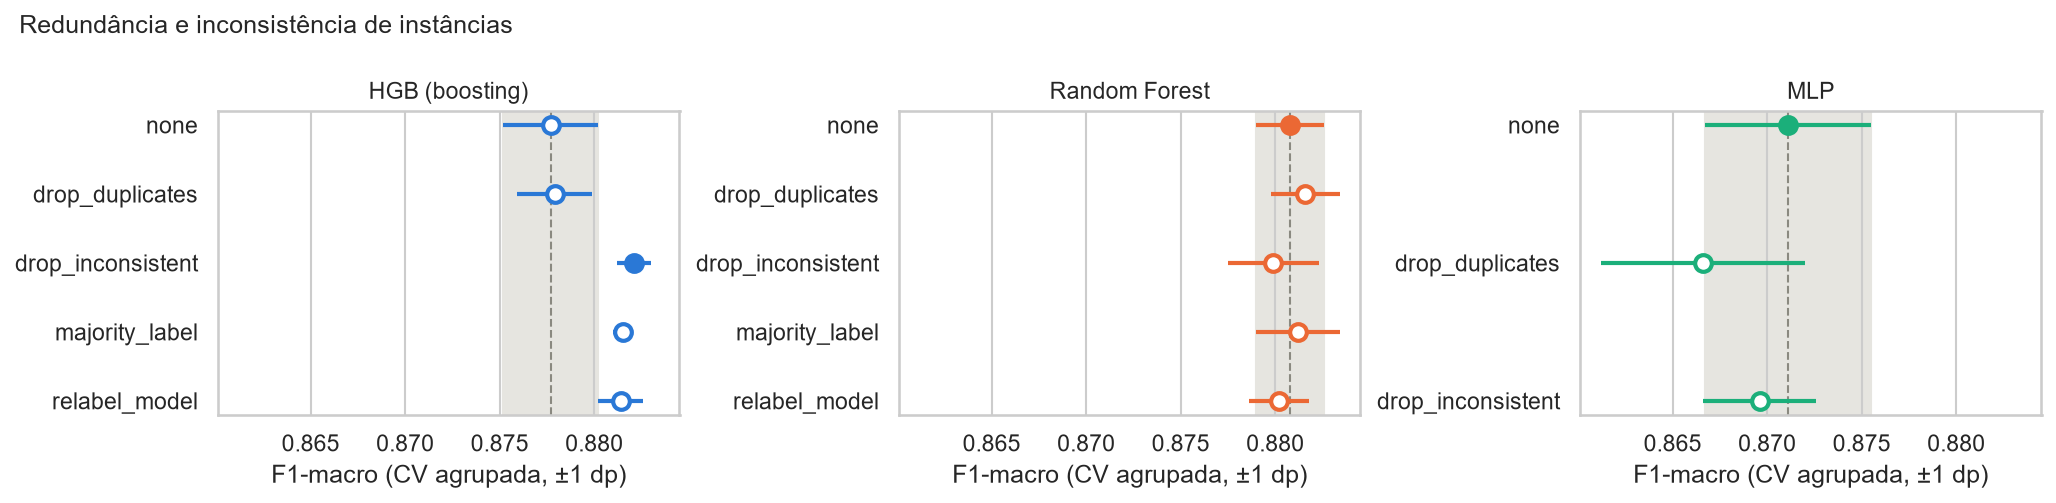
\includegraphics[width=\linewidth,height=0.32\textheight,keepaspectratio]{figuras/pre_redundancia.png}
\caption{F1-macro por estratégia de redundância e inconsistência, em cada família.}
\end{figure}

\textbf{No HGB, a limpeza de rótulos ajuda claramente.} A \texttt{drop\_inconsistent} (0,8821 $\pm$ 0,0009), a \texttt{majority\_label} (0,8815) e a \texttt{relabel\_model} (0,8814) superam a referência \texttt{none} (0,8777 $\pm$ 0,0025) por mais de 1 desvio-padrão. Isso tem uma explicação: no boosting, cada árvore é ajustada aos erros das anteriores, então o modelo insiste em acertar os exemplos com rótulo trocado e acaba memorizando o ruído, o que prejudica também as previsões das linhas vizinhas, sem conflito. Removê-los antes do ajuste corrige o problema. As três limpezas empatam entre si; pela regra, fica a primeira que passa de 1 desvio-padrão e não é superada, a \texttt{drop\_inconsistent}. Note que a limpeza vale mesmo pontuando todas as linhas: os conflitos saem só do \emph{treino} de cada fold, e a validação continua com todos eles.

\textbf{No RF, nenhuma estratégia passa da regra}: todas ficam entre 0,8799 e 0,8816, e por isso mantivemos \texttt{none}. O bagging já é robusto a ruído de rótulo, porque cada árvore vê uma amostra diferente dos dados e o voto final dilui os exemplos trocados.

\textbf{No MLP, também fica \texttt{none}.} Nenhuma limpeza supera a referência (0,8711 $\pm$ 0,0044), e a \texttt{drop\_duplicates} piora.

A \textbf{\texttt{relabel\_model} não compensou} em nenhuma família. Recuperar parte dos conflitos com um modelo não foi melhor do que simplesmente removê-los. É um resultado negativo, mas útil: a informação extra não paga o risco de propagar os erros do próprio modelo.

Já a \texttt{drop\_duplicates} sozinha não muda nada nas árvores. Isso mostra que o problema não são as cópias em si, e sim os rótulos contraditórios.

\section{Valores impossíveis}

A Etapa 1 encontrou valores que não podem existir pela definição dos atributos: taxas maiores que 1, contagens acima da janela do KDD (511 conexões e 255 hosts) e valores negativos em atributos que não podem ser negativos. Eles não têm relação com a classe e parecem erro de medição. Os limites vêm da definição dos atributos, e não de estatísticas da base. Por isso, o tratamento é feito linha a linha e não aprende nada com os dados.

\begin{table}[H]
\centering
\caption{Estratégias para valores impossíveis.}
\begin{tabular}{lp{11cm}}
\toprule
Estratégia & O que faz \\
\midrule
\texttt{nan} & o valor vira ausente e segue para a imputação (referência) \\
\texttt{none} & mantém o valor como está \\
\texttt{clip} & satura no limite (uma taxa de 3,2 vira 1,0; um negativo vira 0) \\
\bottomrule
\end{tabular}
\end{table}

A referência é \texttt{nan} porque não há como recuperar o valor correto: um 600 numa taxa pode ser 6$\times$100 ou 60$\times$10. Saturar no limite inventa um valor, enquanto tratar como ausente admite que ele se perdeu.

\begin{saida}
Linhas com algum valor impossível: 5,674 (8.1%)
Taxa de anomaly nessas linhas: 5.9% (base: 5.8%)
\end{saida}

\begin{table}[H]
\centering
\caption{Atributos com mais valores impossíveis.}
\begin{tabular}{lr}
\toprule
Atributo & valores impossíveis \\
\midrule
dst\_host\_count & 912 \\
dst\_host\_srv\_diff\_host\_rate & 739 \\
dst\_host\_srv\_rerror\_rate & 714 \\
rerror\_rate & 683 \\
dst\_host\_same\_srv\_rate & 670 \\
dst\_host\_diff\_srv\_rate & 623 \\
srv\_count & 507 \\
count & 464 \\
duration & 382 \\
src\_bytes & 189 \\
\bottomrule
\end{tabular}
\end{table}

Os valores impossíveis atingem 8,1\% das linhas, e a taxa de anomalia nelas (5,9\%) é praticamente a mesma da base (5,8\%), o que confirma que não são sinal de ataque.

\begin{table}[H]
\centering
\caption{Resultados da validação cruzada: valores impossíveis.}
\begin{adjustbox}{max width=\linewidth}
\begin{tabular}{llrrrrrrrc}
\toprule
Família & Opção & F1-macro & dp & ganho & sem conflitos & precisão anom. & recall anom. & limiar & escolhida \\
\midrule
HGB & nan & 0.8821 & 0.0009 & 0.0000 & 0.9815 & 0.7565 & 0.8017 & 0.110 & \checkmark \\
HGB & none & 0.8817 & 0.0008 & $-$0.0004 & 0.9810 & 0.7561 & 0.8007 & 0.114 &  \\
HGB & clip & 0.8814 & 0.0010 & $-$0.0007 & 0.9816 & 0.7601 & 0.7946 & 0.210 &  \\
\midrule
MLP & nan & 0.8711 & 0.0044 & 0.0000 & 0.9643 & 0.7456 & 0.7705 & 0.344 & \checkmark \\
MLP & none & 0.8681 & 0.0025 & $-$0.0030 & 0.9590 & 0.7406 & 0.7642 & 0.346 &  \\
MLP & clip & 0.8699 & 0.0032 & $-$0.0012 & 0.9617 & 0.7417 & 0.7700 & 0.332 &  \\
\bottomrule
\end{tabular}
\end{adjustbox}
\end{table}

\begin{figure}[H]
\centering
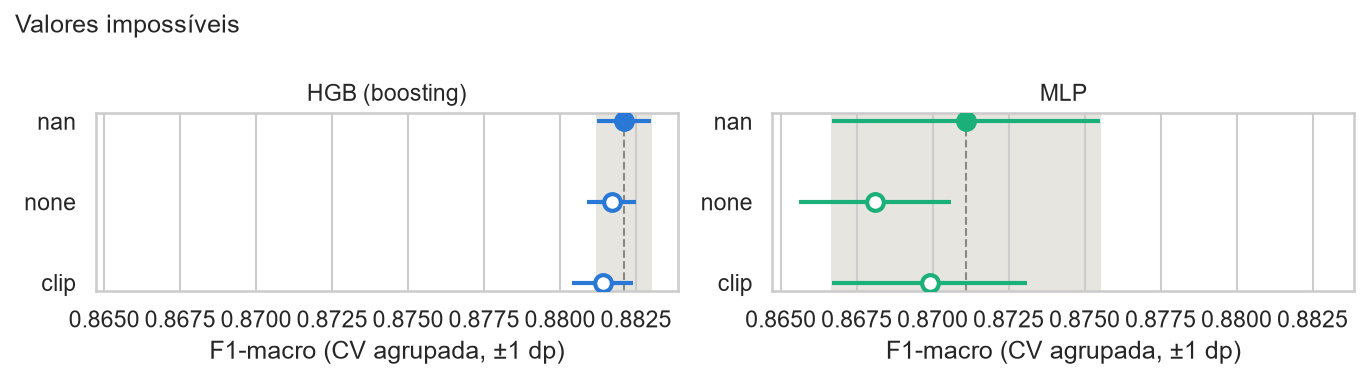
\includegraphics[width=\linewidth,height=0.25\textheight,keepaspectratio]{figuras/pre_dominio.png}
\caption{F1-macro por tratamento de valores impossíveis.}
\end{figure}

A opção \texttt{nan} foi a melhor nas duas famílias testadas (HGB 0,8821; MLP 0,8711). No HGB, \texttt{none} e \texttt{clip} perdem menos de 0,001, dentro do ruído. No MLP, \texttt{clip} empata, mas manter o valor (\texttt{none}) custa 0,003. Isso acontece porque um valor como 600 numa taxa vira, depois da padronização, um ponto extremo que distorce os pesos da rede.

O RF não foi testado neste eixo. O comportamento das árvores já estava coberto pelo HGB, e a regra manteria a referência de qualquer forma. Assim, \texttt{nan} vale para todas as famílias.

\section{Valores ausentes}

Quase todas as linhas (94\%) têm algum valor ausente, com até 40\% de falta em \texttt{src\_bytes}. Descartar linhas é inviável, e o teste também tem ausentes, então o modelo precisa saber lidar com eles. Comparamos cinco estratégias:

\begin{table}[H]
\centering
\caption{Estratégias de imputação.}
\begin{tabular}{lp{11cm}}
\toprule
Estratégia & O que faz \\
\midrule
\texttt{none} & NaN nativo: o HGB aprende para que lado de cada divisão o ausente deve ir (só para árvores) \\
\texttt{mean}, \texttt{median} & substitui pela média ou pela mediana do fold de treino \\
\texttt{median\_indicator} & mediana e mais uma coluna binária ``estava ausente'' por atributo \\
\texttt{iterative} & estima cada atributo a partir dos outros (MICE, \texttt{IterativeImputer}) \\
\bottomrule
\end{tabular}
\end{table}

Nos atributos categóricos, o ausente vira a categoria \texttt{ausente}, em todas as estratégias.

A Etapa 1 mostrou que a falta em \texttt{dst\_host\_serror\_rate} é MNAR: os valores altos somem mais, e um valor alto indica ataque. A mediana apaga esse sinal, enquanto o NaN nativo e o indicador o preservam. Por isso, esperávamos alguma vantagem dessas duas opções.

\begin{saida}
Atributos com ausentes: 24 | linhas com algum ausente: 93.8%
dst_host_serror_rate: taxa de anomaly com ausente 8.5% × sem ausente 4.6%
\end{saida}

\begin{table}[H]
\centering
\caption{Atributos com maior percentual de ausentes.}
\begin{tabular}{lr}
\toprule
Atributo & \% ausente \\
\midrule
src\_bytes & 40,0 \\
dst\_host\_srv\_count & 39,9 \\
dst\_host\_serror\_rate & 30,6 \\
dst\_host\_same\_src\_port\_rate & 28,0 \\
serror\_rate & 6,8 \\
service & 6,3 \\
logged\_in & 6,1 \\
srv\_diff\_host\_rate & 6,1 \\
\bottomrule
\end{tabular}
\end{table}

\begin{table}[H]
\centering
\caption{Resultados da validação cruzada: imputação de ausentes.}
\begin{adjustbox}{max width=\linewidth}
\begin{tabular}{llrrrrrrrc}
\toprule
Família & Opção & F1-macro & dp & ganho & sem conflitos & precisão anom. & recall anom. & limiar & escolhida \\
\midrule
HGB & none & 0.8821 & 0.0009 & 0.0000 & 0.9815 & 0.7565 & 0.8017 & 0.110 & \checkmark \\
HGB & median & 0.8817 & 0.0005 & $-$0.0004 & 0.9812 & 0.7566 & 0.8000 & 0.172 &  \\
HGB & median\_indicator & 0.8814 & 0.0013 & $-$0.0007 & 0.9804 & 0.7568 & 0.7985 & 0.174 &  \\
\midrule
RF & median & 0.8808 & 0.0018 & 0.0000 & 0.9786 & 0.7534 & 0.8002 & 0.308 & \checkmark \\
RF & none & 0.8809 & 0.0022 & 0.0001 & 0.9783 & 0.7511 & 0.8031 & 0.284 &  \\
RF & median\_indicator & 0.8807 & 0.0027 & $-$0.0001 & 0.9784 & 0.7530 & 0.8002 & 0.290 &  \\
RF & mean & 0.8811 & 0.0020 & 0.0003 & 0.9788 & 0.7526 & 0.8022 & 0.288 &  \\
\midrule
MLP & median & 0.8711 & 0.0044 & 0.0000 & 0.9643 & 0.7456 & 0.7705 & 0.344 & \checkmark \\
MLP & mean & 0.8692 & 0.0039 & $-$0.0019 & 0.9589 & 0.7365 & 0.7732 & 0.290 &  \\
MLP & median\_indicator & 0.8594 & 0.0051 & $-$0.0117 & 0.9455 & 0.7321 & 0.7392 & 0.344 &  \\
MLP & iterative & 0.8685 & 0.0045 & $-$0.0026 & 0.9582 & 0.7388 & 0.7678 & 0.306 &  \\
\bottomrule
\end{tabular}
\end{adjustbox}
\end{table}

\begin{figure}[H]
\centering
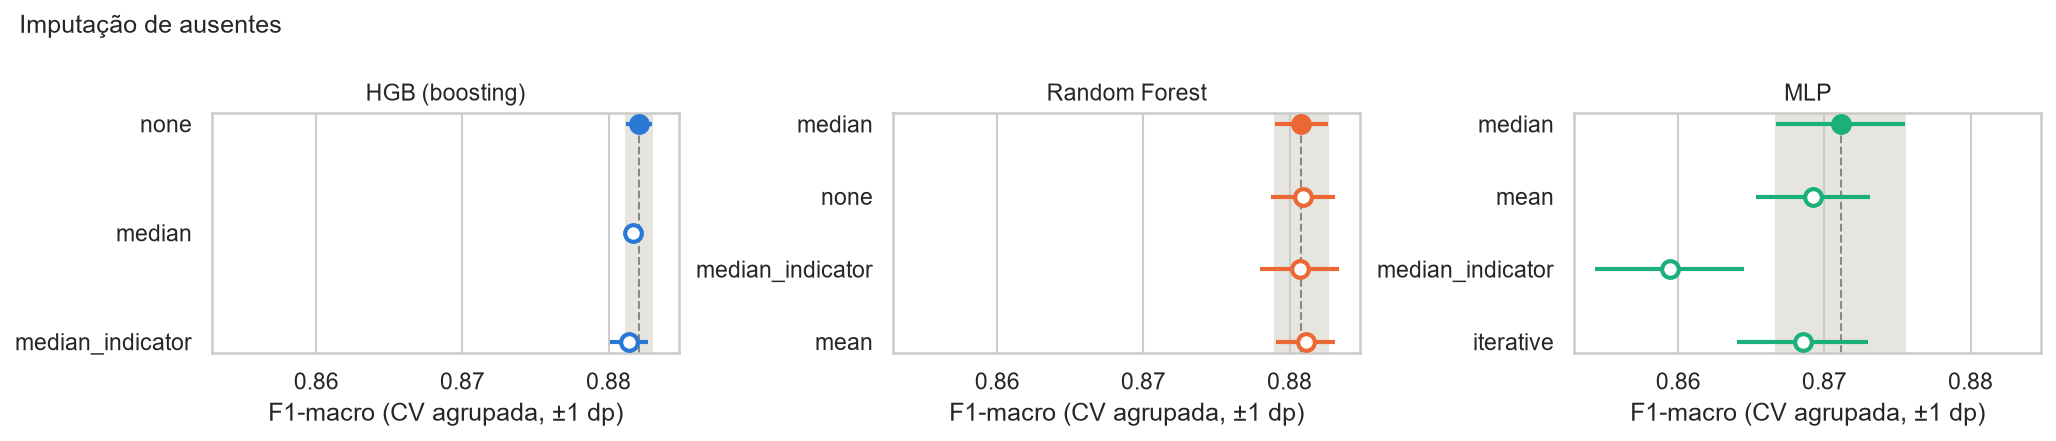
\includegraphics[width=\linewidth,height=0.30\textheight,keepaspectratio]{figuras/pre_imputacao.png}
\caption{F1-macro por estratégia de imputação.}
\end{figure}

\textbf{No HGB}, o NaN nativo (0,8821) fica à frente da mediana (0,8817) e do indicador (0,8814). Nenhuma imputação supera a referência, e o NaN nativo é o mais simples: o próprio modelo aprende o que a ausência significa em cada atributo.

\textbf{No RF}, as quatro opções empatam (de 0,8807 a 0,8811), e por isso fica a mediana, que é a referência dessa família.

\textbf{No MLP}, a mediana (0,8711) fica à frente. A média (0,8692) e a imputação iterativa (0,8685) perdem pouco, mas o indicador perde 0,012. O indicador dobra o número de colunas numéricas com sinais binários fracos, e a rede acaba se ajustando a ruído.

O indicador de ausência \textbf{não melhorou em nenhuma família}, apesar do padrão MNAR de \texttt{dst\_host\_serror\_rate}. Provavelmente, o sinal da ausência nesse atributo é pequeno perto do que os outros 40 atributos já informam. Registramos o resultado mesmo assim, porque ele contraria a expectativa que tínhamos na Etapa 1.

\section{Codificação simbólico-numérica de \texttt{service} (requisito 3)}

Os atributos \texttt{protocol\_type} (3 valores) e \texttt{flag} (11 valores) têm poucas categorias e usam one-hot, ou a codificação nativa no HGB. O desafio está em \texttt{service}: são 67 categorias depois de padronizar a grafia (68 contando a categoria \texttt{ausente}), com uma cauda longa de serviços raros.

\begin{saida}
Categorias de service: 68 | as 5 maiores cobrem 84.0% das linhas
Categorias com < 0,1% das linhas (agrupadas por onehot_rare): 50
Taxa de anomaly por categoria: de 0% a 100%
\end{saida}

\begin{table}[H]
\centering
\caption{As 8 categorias mais frequentes de \texttt{service}.}
\begin{tabular}{lrr}
\toprule
service & \% das linhas & \% de anomaly \\
\midrule
http & 51,9 & 1,7 \\
domain\_u & 11,0 & 1,0 \\
smtp & 8,7 & 1,3 \\
ausente & 6,3 & 6,2 \\
ftp\_data & 6,1 & 3,0 \\
private & 4,2 & 40,0 \\
other & 3,1 & 5,9 \\
ftp & 1,6 & 6,1 \\
\bottomrule
\end{tabular}
\end{table}

A distribuição é muito concentrada: cinco serviços cobrem 84\% das linhas, e 50 categorias têm menos de 0,1\% cada. A taxa de anomalia varia de 0\% a 100\% entre as categorias. O caso mais marcante é o \texttt{private}, com 40\% de anomalias contra menos de 2\% no \texttt{http}.

Comparamos as seguintes codificações, cada uma com uma suposição diferente:

\begin{table}[H]
\centering
\caption{Codificações comparadas para \texttt{service}.}
\begin{adjustbox}{max width=\linewidth}
\begin{tabular}{lcp{10cm}}
\toprule
Codificação & Colunas & Prós e contras \\
\midrule
\texttt{onehot} & 67 & não impõe ordem (a distância de Hamming entre categorias é constante), mas cria muitas colunas esparsas \\
\texttt{onehot\_rare} & $\sim$19 & one-hot em que as categorias com menos de 0,1\% das linhas são reunidas numa coluna ``rara'' \\
\texttt{frequency} & 1 & pseudoatributo com a fração de linhas da categoria; categorias diferentes com a mesma frequência se confundem \\
\texttt{target} & 1 & pseudoatributo com a taxa de \texttt{anomaly} da categoria, calculada com \emph{cross-fitting} interno para não vazar o rótulo \\
\texttt{ordinal} & 1 & um número inteiro arbitrário por categoria; impõe uma ordem falsa, aceitável só para árvores \\
nativa (HGB) & 1 & o HGB divide as categorias em grupos sem supor nenhuma ordem \\
\bottomrule
\end{tabular}
\end{adjustbox}
\end{table}

O material da disciplina alerta que a codificação 1-de-$c$ não é uma boa opção quando há muitas categorias (o exemplo dos ``193 países'') e sugere o uso de pseudoatributos. Por isso, colocamos \texttt{frequency} e \texttt{target} para competir com o one-hot. O HGB usa a codificação nativa e não entra neste eixo.

\begin{table}[H]
\centering
\caption{Resultados da validação cruzada: codificação de \texttt{service}.}
\begin{adjustbox}{max width=\linewidth}
\begin{tabular}{llrrrrrrrc}
\toprule
Família & Opção & F1-macro & dp & ganho & sem conflitos & precisão anom. & recall anom. & limiar & escolhida \\
\midrule
RF & onehot & 0.8808 & 0.0018 & 0.0000 & 0.9786 & 0.7534 & 0.8002 & 0.308 & \checkmark \\
RF & onehot\_rare & 0.8812 & 0.0010 & 0.0004 & 0.9808 & 0.7570 & 0.7973 & 0.332 &  \\
RF & frequency & 0.8803 & 0.0017 & $-$0.0005 & 0.9790 & 0.7563 & 0.7946 & 0.340 &  \\
RF & target & 0.8800 & 0.0015 & $-$0.0008 & 0.9773 & 0.7520 & 0.7985 & 0.320 &  \\
RF & ordinal & 0.8801 & 0.0011 & $-$0.0007 & 0.9778 & 0.7522 & 0.7987 & 0.316 &  \\
\midrule
MLP & onehot & 0.8711 & 0.0044 & 0.0000 & 0.9643 & 0.7456 & 0.7705 & 0.344 & \checkmark \\
MLP & onehot\_rare & 0.8730 & 0.0022 & 0.0019 & 0.9640 & 0.7389 & 0.7852 & 0.354 &  \\
MLP & frequency & 0.8675 & 0.0059 & $-$0.0036 & 0.9563 & 0.7332 & 0.7696 & 0.324 &  \\
MLP & target & 0.8651 & 0.0060 & $-$0.0060 & 0.9510 & 0.7288 & 0.7659 & 0.270 &  \\
\bottomrule
\end{tabular}
\end{adjustbox}
\end{table}

\begin{figure}[H]
\centering
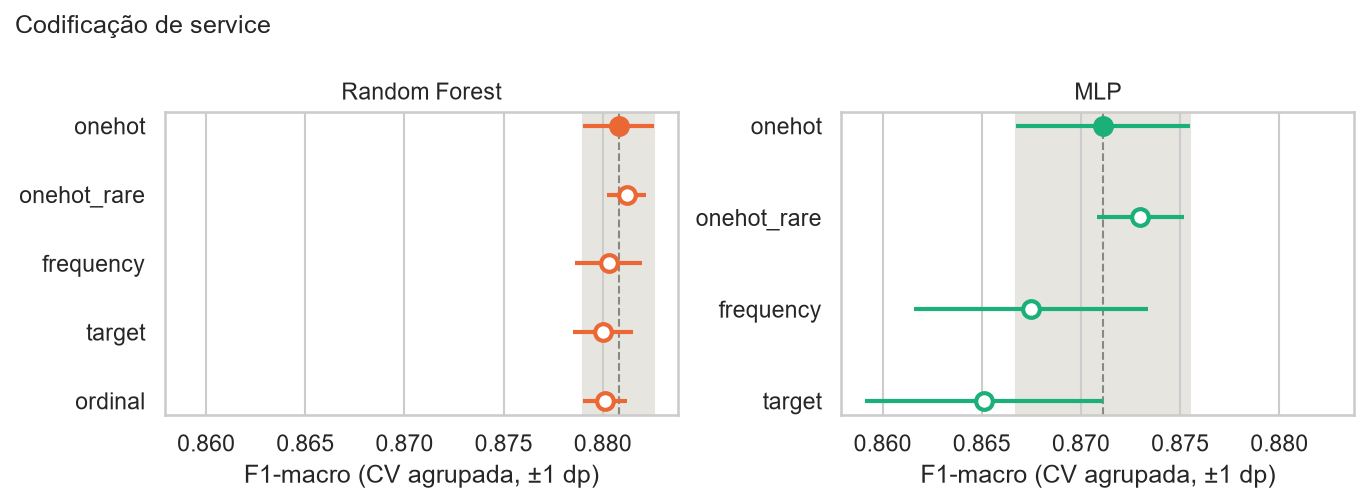
\includegraphics[width=\linewidth,height=0.28\textheight,keepaspectratio]{figuras/pre_codificacao.png}
\caption{F1-macro por codificação de \texttt{service}.}
\end{figure}

\textbf{No RF}, as cinco opções empatam dentro de 1 desvio-padrão (de 0,8800 a 0,8812), e fica o \texttt{onehot}, que é a referência. O \texttt{target} é o pior: resumir 67 categorias num único número esconde combinações, como \texttt{service} $\times$ \texttt{flag}, que as árvores conseguem aproveitar no one-hot.

\textbf{No MLP}, o \texttt{onehot\_rare} tem a maior média (0,8730), mas o ganho (0,0019) fica abaixo de 1 desvio-padrão (0,0044), e por isso fica o \texttt{onehot}. A \texttt{frequency} (0,8675) e o \texttt{target} (0,8651) perdem. Para a rede, uma única coluna numérica força uma relação monotônica entre a categoria e a saída, e essa relação não existe: serviços com frequência parecida podem ter perfis de ataque opostos.

O alerta do material sobre alta cardinalidade \textbf{se confirma só em parte}. A cauda de fato é longa, com 50 categorias abaixo de 0,1\% das linhas cada, mas essas colunas raras quase não pesam: reuni-las (\texttt{onehot\_rare}) não muda o resultado além do ruído. Com 70 mil linhas, as 67 colunas esparsas não atrapalham os modelos, e o one-hot preserva toda a informação sem criar uma ordem falsa.

\section{Balanceamento de classes (requisito 2)}

Apenas 5,8\% das linhas são \texttt{anomaly}, uma proporção de 16 para 1. O material da disciplina resume bem o dilema: o \emph{oversampling} arrisca sobreajuste e a criação de instâncias irreais, enquanto o \emph{undersampling} arrisca perder informação. Batista et al. (2004) recomendam SMOTE com Tomek quando há poucos exemplos positivos. Comparamos sete técnicas com a opção de não balancear:

\begin{table}[H]
\centering
\caption{Técnicas de balanceamento (todas aplicadas só no fold de treino).}
\begin{adjustbox}{max width=\linewidth}
\begin{tabular}{lp{11cm}}
\toprule
Técnica & O que faz \\
\midrule
\texttt{class\_weight} & não reamostra; dá mais peso aos erros na classe rara (RF e HGB) \\
\texttt{ros} & replica linhas de \texttt{anomaly} até chegar a 10.000 \\
\texttt{rus} & reduz as linhas de \texttt{normal} para 10.000 \\
\texttt{smote} & cria linhas sintéticas de \texttt{anomaly}, interpolando entre vizinhos, até 10.000 \\
\texttt{borderline\_smote} & SMOTE gerado só a partir dos positivos que estão perto da fronteira entre as classes \\
\texttt{smote\_tomek} & SMOTE seguido da remoção dos pares de Tomek, que limpa a fronteira \\
\texttt{hybrid} & RUS de \texttt{normal} até 20.000 e SMOTE de \texttt{anomaly} até 5.000 \\
\bottomrule
\end{tabular}
\end{adjustbox}
\end{table}

O balanceador é o último passo antes do modelo, dentro do pipeline. Ele só reamostra durante o ajuste (\texttt{fit}), então as linhas de validação nunca ganham nem perdem instâncias. Como precisa de dados completos, ele roda depois da imputação. No HGB, que usa NaN nativo, só o \texttt{class\_weight} é possível.

\begin{table}[H]
\centering
\caption{Resultados da validação cruzada: balanceamento.}
\begin{adjustbox}{max width=\linewidth}
\begin{tabular}{llrrrrrrrc}
\toprule
Família & Opção & F1-macro & dp & ganho & sem conflitos & precisão anom. & recall anom. & limiar & escolhida \\
\midrule
HGB & none & 0.8821 & 0.0009 & 0.0000 & 0.9815 & 0.7565 & 0.8017 & 0.110 & \checkmark \\
HGB & class\_weight & 0.8807 & 0.0014 & $-$0.0014 & 0.9799 & 0.7582 & 0.7941 & 0.606 &  \\
\midrule
RF & none & 0.8808 & 0.0018 & 0.0000 & 0.9786 & 0.7534 & 0.8002 & 0.308 & \checkmark \\
RF & class\_weight & 0.8763 & 0.0012 & $-$0.0045 & 0.9710 & 0.7469 & 0.7897 & 0.524 &  \\
RF & ros (10.000) & 0.8799 & 0.0016 & $-$0.0009 & 0.9762 & 0.7493 & 0.8012 & 0.382 &  \\
RF & rus (10.000) & 0.8746 & 0.0027 & $-$0.0062 & 0.9690 & 0.7497 & 0.7794 & 0.628 &  \\
RF & smote (10.000) & 0.8807 & 0.0014 & $-$0.0001 & 0.9787 & 0.7541 & 0.7987 & 0.372 &  \\
RF & borderline\_smote (10.000) & 0.8810 & 0.0026 & 0.0002 & 0.9773 & 0.7504 & 0.8041 & 0.352 &  \\
RF & smote\_tomek (10.000) & 0.8816 & 0.0011 & 0.0008 & 0.9796 & 0.7543 & 0.8022 & 0.354 &  \\
RF & hybrid (5.000 / 20.000) & 0.8794 & 0.0019 & $-$0.0014 & 0.9761 & 0.7512 & 0.7968 & 0.498 &  \\
\midrule
MLP & none & 0.8711 & 0.0044 & 0.0000 & 0.9643 & 0.7456 & 0.7705 & 0.344 & \checkmark \\
MLP & ros (10.000) & 0.8693 & 0.0025 & $-$0.0018 & 0.9605 & 0.7409 & 0.7683 & 0.640 &  \\
MLP & rus (10.000) & 0.8664 & 0.0017 & $-$0.0047 & 0.9512 & 0.7229 & 0.7772 & 0.644 &  \\
MLP & smote (10.000) & 0.8680 & 0.0022 & $-$0.0031 & 0.9565 & 0.7330 & 0.7720 & 0.552 &  \\
MLP & borderline\_smote (10.000) & 0.8548 & 0.0068 & $-$0.0163 & 0.9315 & 0.7045 & 0.7514 & 0.572 &  \\
MLP & smote\_tomek (10.000) & 0.8702 & 0.0035 & $-$0.0009 & 0.9591 & 0.7341 & 0.7794 & 0.520 &  \\
MLP & hybrid (5.000 / 20.000) & 0.8704 & 0.0026 & $-$0.0007 & 0.9598 & 0.7357 & 0.7786 & 0.544 &  \\
\bottomrule
\end{tabular}
\end{adjustbox}
\end{table}

\begin{figure}[H]
\centering
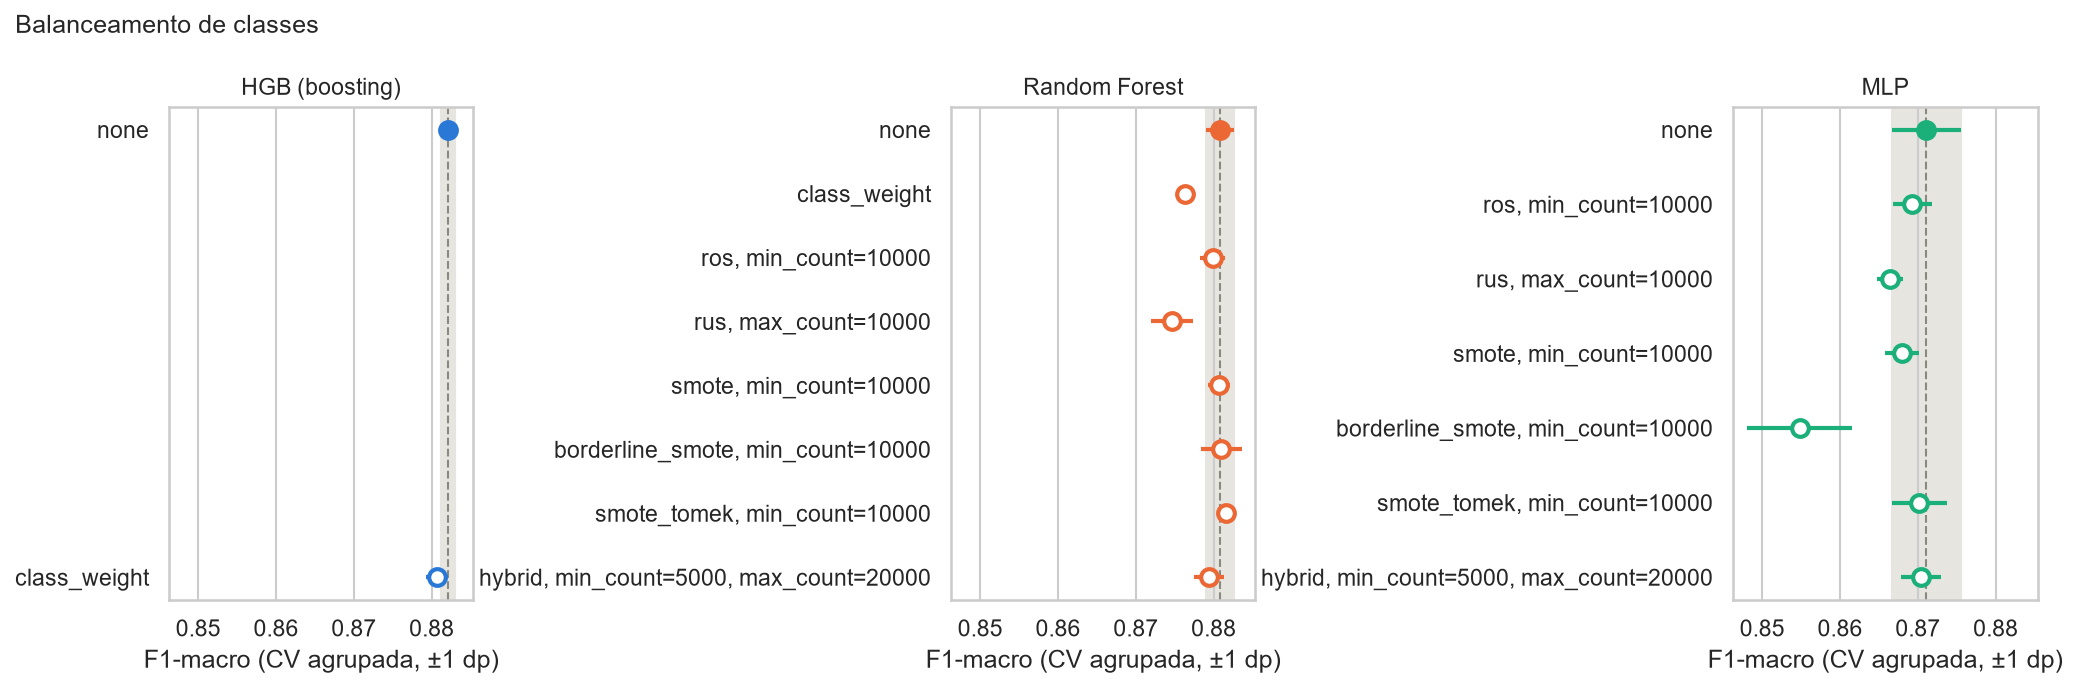
\includegraphics[width=\linewidth,height=0.32\textheight,keepaspectratio]{figuras/pre_balanceamento.png}
\caption{F1-macro por técnica de balanceamento.}
\end{figure}

\textbf{Nenhuma técnica supera a opção de não balancear}, em nenhuma família. No RF, o SMOTE com Tomek (0,8816) fica um pouco à frente da referência (0,8808 $\pm$ 0,0018), mas dentro do ruído. Por isso, a escolha foi \texttt{none}.

O \textbf{RUS piora} no RF e no MLP. Descartar cerca de 80\% das linhas \texttt{normal} faz o modelo perder informação sobre o tráfego legítimo, e os falsos positivos aumentam, como mostra a queda da precisão. O \texttt{class\_weight} também piora no RF.

\textbf{Por que balancear não ajuda aqui?} O F1-macro é calculado depois de escolher o limiar de decisão nas previsões \emph{out-of-fold}. Reamostrar muda a probabilidade que o modelo atribui à classe \texttt{anomaly}, mas o limiar ajustado já desloca a fronteira para o ponto que maximiza o F1-macro. A coluna \emph{limiar} mostra isso: com ROS ou SMOTE, o limiar sobe (no RF, de 0,31 para 0,38 e 0,37), compensando a probabilidade inflada. Em resumo, o balanceamento e o ajuste do limiar resolvem o mesmo problema, mas o limiar faz isso sem distorcer os dados de treino.

Há ainda uma \textbf{limitação do SMOTE} nesta base. Ele roda depois do one-hot e interpola também as colunas binárias, gerando valores fracionários (algo como ``meio \texttt{http}, meio \texttt{ftp}'') que não existem em conexões reais. Isso explica parte do resultado fraco no MLP, sobretudo o do \texttt{borderline\_smote} (0,8548).

\section{Normalização e transformação numérica (requisito 4)}

Os volumes (\texttt{src\_bytes}, \texttt{dst\_bytes}, \texttt{duration}) e as contagens têm cauda muito longa. Para modelos que dependem de distâncias ou de gradientes, como o MLP, a escala dos atributos importa. Medimos a assimetria antes e depois de aplicar o \texttt{log1p} (com sinal) nos atributos de cauda longa (\texttt{config.HEAVY\_TAILED}). Essa transformação é fixa, aplicada valor a valor, sem nenhum parâmetro aprendido.

\begin{table}[H]
\centering
\caption{Assimetria antes e depois do \texttt{log1p}, nos 8 atributos mais assimétricos.}
\begin{tabular}{lrr}
\toprule
Atributo & assimetria original & assimetria após log1p \\
\midrule
dst\_bytes & 237,2 & $-$0,5 \\
num\_root & 187,5 & 21,7 \\
duration & 163,4 & 4,2 \\
src\_bytes & 96,9 & $-$1,4 \\
num\_file\_creations & 69,2 & 28,7 \\
count & 61,2 & 1,2 \\
srv\_count & 57,6 & 1,3 \\
num\_compromised & 55,1 & 9,0 \\
\bottomrule
\end{tabular}
\end{table}

O \texttt{log1p} praticamente elimina a assimetria nos volumes e nas contagens de conexões. Ela continua alta em \texttt{num\_root} e \texttt{num\_file\_creations}, que são quase sempre zero: nesses atributos, a cauda é feita de poucos valores diferentes de zero, e nenhuma transformação monotônica muda isso.

Comparamos as seguintes opções no MLP:

\begin{table}[H]
\centering
\caption{Opções de normalização e transformação.}
\begin{adjustbox}{max width=\linewidth}
\begin{tabular}{lp{10cm}}
\toprule
Opção & O que faz \\
\midrule
\texttt{standard} + log1p & \texttt{log1p} nos atributos de cauda longa e padronização (média 0, desvio 1) --- referência \\
\texttt{standard} sem log1p & só a padronização \\
\texttt{minmax} + log1p & \texttt{log1p} e escala para o intervalo [0, 1] \\
\texttt{robust} + log1p & \texttt{log1p} e escala pela mediana e pelo intervalo interquartil \\
\texttt{quantile} sem log1p & transforma cada atributo numa distribuição normal, usando os quantis \\
\bottomrule
\end{tabular}
\end{adjustbox}
\end{table}

As árvores (HGB e RF) dividem os dados por limiares e não se alteram com transformações monotônicas: padronizar ou aplicar \texttt{log1p} não muda nenhuma divisão possível. Por isso, este eixo só foi testado no MLP, e nas árvores a escala ficou em \texttt{none}.

\begin{table}[H]
\centering
\caption{Resultados da validação cruzada: normalização e transformação (MLP).}
\begin{adjustbox}{max width=\linewidth}
\begin{tabular}{llrrrrrrrc}
\toprule
Família & Opção & F1-macro & dp & ganho & sem conflitos & precisão anom. & recall anom. & limiar & escolhida \\
\midrule
MLP & standard + log1p & 0.8711 & 0.0044 & 0.0000 & 0.9643 & 0.7456 & 0.7705 & 0.344 & \checkmark \\
MLP & standard sem log1p & 0.8654 & 0.0033 & $-$0.0057 & 0.9545 & 0.7351 & 0.7593 & 0.334 &  \\
MLP & minmax + log1p & 0.8669 & 0.0057 & $-$0.0042 & 0.9585 & 0.7443 & 0.7553 & 0.284 &  \\
MLP & robust + log1p & 0.8623 & 0.0072 & $-$0.0088 & 0.9469 & 0.7248 & 0.7595 & 0.288 &  \\
MLP & quantile sem log1p & 0.8646 & 0.0045 & $-$0.0065 & 0.9531 & 0.7356 & 0.7561 & 0.374 &  \\
\bottomrule
\end{tabular}
\end{adjustbox}
\end{table}

\begin{figure}[H]
\centering
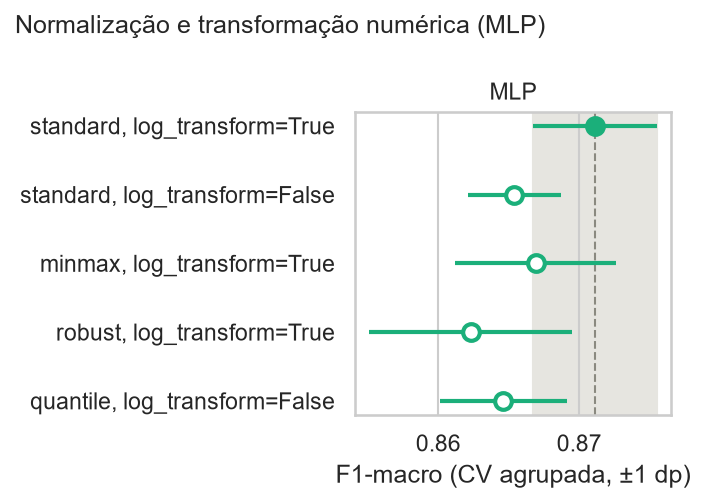
\includegraphics[width=0.55\linewidth,height=0.25\textheight,keepaspectratio]{figuras/pre_escala.png}
\caption{F1-macro por normalização e transformação numérica (MLP).}
\end{figure}

O \texttt{log1p} seguido de padronização foi a melhor opção (0,8711 $\pm$ 0,0044). Sem o \texttt{log1p}, o resultado cai para 0,8654. Com assimetrias acima de 100, a padronização sozinha deixa quase todas as linhas espremidas perto de zero e algumas poucas em valores enormes, e a rede não consegue separar o tráfego comum.

O \texttt{minmax} (0,8669) sofre do mesmo problema, porque o máximo é definido por poucas linhas extremas. O \texttt{robust} foi o pior (0,8623): em atributos com mais da metade dos valores iguais a zero, o intervalo interquartil é zero ou quase zero, e a escala explode. Já o \texttt{quantile} (0,8646) resolve a cauda, mas achata as diferenças entre os valores grandes, que são justamente as que separam alguns ataques de volume.

\section{Redução de dimensionalidade (requisito 5)}

Depois do one-hot, o RF e o MLP recebem cerca de 120 colunas, e a Etapa 1 mostrou grupos de atributos muito correlacionados, como as taxas de \texttt{serror} e \texttt{rerror}. Comparamos:

\begin{table}[H]
\centering
\caption{Técnicas de redução de dimensionalidade.}
\begin{adjustbox}{max width=\linewidth}
\begin{tabular}{lp{11cm}}
\toprule
Técnica & O que faz \\
\midrule
\texttt{none} & usa todas as colunas (referência) \\
\texttt{pca} & componentes principais que explicam 95\% da variância \\
\texttt{kbest\_f} & as 30 colunas com maior estatística F (ANOVA) em relação à classe \\
\texttt{kbest\_mi} & as 30 colunas com maior informação mútua com a classe \\
\texttt{tree\_select} & as colunas com importância acima da mediana num ExtraTrees ajustado no fold \\
\bottomrule
\end{tabular}
\end{adjustbox}
\end{table}

O enunciado permite escolher entre redução de dimensionalidade e seleção de instâncias, e optamos pela redução. A seleção de instâncias por limpeza da fronteira já aparece no eixo de balanceamento (\texttt{smote\_tomek}), e a remoção de redundâncias, na Seção 2.

\begin{table}[H]
\centering
\caption{Resultados da validação cruzada: redução de dimensionalidade.}
\begin{adjustbox}{max width=\linewidth}
\begin{tabular}{llrrrrrrrc}
\toprule
Família & Opção & F1-macro & dp & ganho & sem conflitos & precisão anom. & recall anom. & limiar & escolhida \\
\midrule
RF & none & 0.8808 & 0.0018 & 0.0000 & 0.9786 & 0.7534 & 0.8002 & 0.308 & \checkmark \\
RF & pca & 0.7201 & 0.0537 & $-$0.1607 & 0.7393 & 0.4704 & 0.5013 & 0.318 &  \\
RF & kbest\_f (k = 30) & 0.8639 & 0.0043 & $-$0.0169 & 0.9539 & 0.7416 & 0.7465 & 0.402 &  \\
RF & kbest\_mi (k = 30) & 0.8785 & 0.0030 & $-$0.0023 & 0.9755 & 0.7522 & 0.7921 & 0.310 &  \\
RF & tree\_select & 0.8819 & 0.0016 & 0.0011 & 0.9807 & 0.7551 & 0.8024 & 0.318 &  \\
\midrule
MLP & none & 0.8711 & 0.0044 & 0.0000 & 0.9643 & 0.7456 & 0.7705 & 0.344 & \checkmark \\
MLP & pca & 0.8655 & 0.0031 & $-$0.0056 & 0.9508 & 0.7257 & 0.7703 & 0.312 &  \\
MLP & kbest\_f (k = 30) & 0.8600 & 0.0096 & $-$0.0111 & 0.9481 & 0.7410 & 0.7325 & 0.378 &  \\
MLP & kbest\_mi (k = 30) & 0.8641 & 0.0063 & $-$0.0070 & 0.9520 & 0.7341 & 0.7556 & 0.328 &  \\
MLP & tree\_select & 0.8724 & 0.0017 & 0.0013 & 0.9639 & 0.7407 & 0.7808 & 0.362 &  \\
\bottomrule
\end{tabular}
\end{adjustbox}
\end{table}

\begin{figure}[H]
\centering
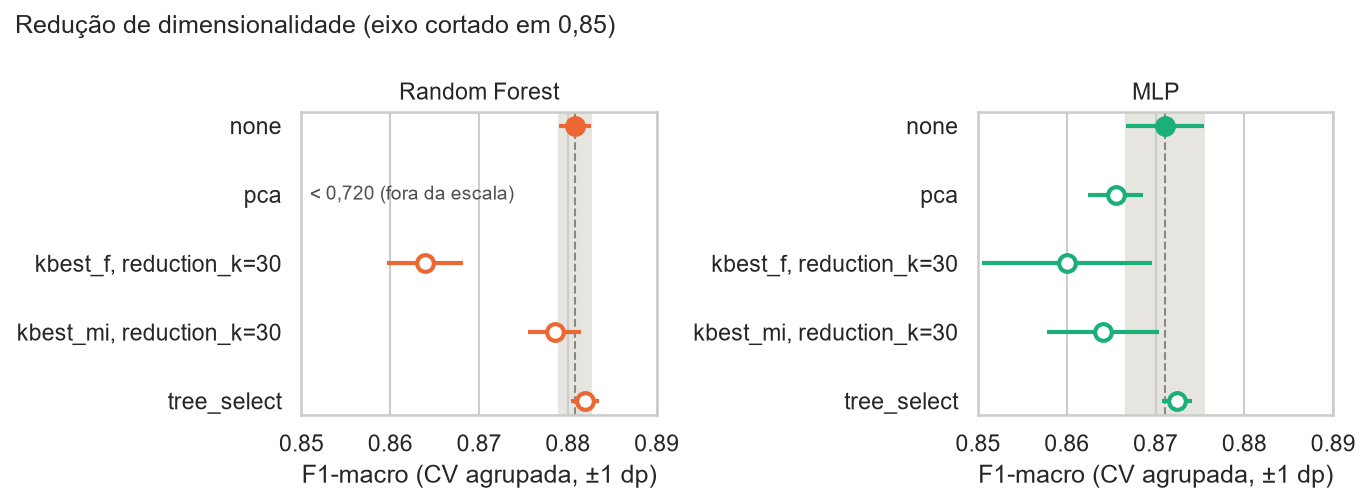
\includegraphics[width=\linewidth,height=0.28\textheight,keepaspectratio]{figuras/pre_reducao.png}
\caption{F1-macro por técnica de redução. O eixo foi cortado em 0,85 para que as diferenças entre as demais opções fiquem visíveis; o PCA no RF (0,720) aparece indicado fora da escala.}
\end{figure}

\subsection{O PCA no Random Forest}

O resultado do PCA no RF (0,72) é um \textbf{artefato da comparação, e não da técnica}. O RF trabalha sem escala (\texttt{scaling="none"}), e um PCA sem padronização é dominado pelos atributos de maior variância. Os volumes \texttt{src\_bytes} e \texttt{dst\_bytes}, na casa dos milhões, ocupam os primeiros componentes, e as taxas, que ficam entre 0 e 1, praticamente desaparecem. Para fazer uma comparação justa, rodamos o PCA no RF com os dados padronizados e com \texttt{log1p}, como no MLP:

\begin{table}[H]
\centering
\caption{RF com padronização e \texttt{log1p}: sem redução $\times$ PCA.}
\begin{tabular}{lrrr}
\toprule
Opção & F1-macro & dp & sem conflitos \\
\midrule
none & 0.8815 & 0.0017 & 0.9802 \\
pca & 0.8686 & 0.0026 & 0.9588 \\
\bottomrule
\end{tabular}
\end{table}

\subsection{O que concluímos}

Com os dados padronizados, o PCA no RF deixa de ser um desastre, mas ainda perde para a opção sem redução (0,8686 contra 0,8815). No MLP, ele também perde (0,8655 contra 0,8711). O PCA combina os atributos nas direções de \textbf{maior variância}, que não são necessariamente as que separam as classes. Além disso, o RF deixa de poder dividir os dados por um atributo original de cada vez.

O \texttt{kbest\_f} e o \texttt{kbest\_mi}, com 30 colunas, perdem nas duas famílias. O critério deles é univariado: avalia cada coluna isoladamente e descarta as que só ajudam em combinação com outras, como as categorias de \texttt{service} que importam apenas junto com certas \texttt{flag}.

O \textbf{\texttt{tree\_select} é a única técnica que não perde, mas não passa da regra}. No RF, chega a 0,8819 $\pm$ 0,0016, contra 0,8808 $\pm$ 0,0018 sem redução, um ganho de 0,0011, abaixo de 1 desvio-padrão. No MLP, também empata (0,8724 contra 0,8711). A seleção por árvores avalia as colunas em conjunto e mantém só as que têm importância acima da mediana; as descartadas, como as colunas de serviços raros, quase não são usadas pelas árvores, e por isso ela não perde nada.

Pela regra, ficamos sem redução nas duas famílias. Como o \texttt{tree\_select} no RF ficou perto da regra, a Seção 9 confere com mais repetições se ele esconde um ganho real.

\section{Robustez das escolhas (validação cruzada repetida 3$\times$5)}

A busca por coordenadas faz muitas comparações seguidas, e as diferenças são de milésimos. Repetimos a validação cruzada 3 vezes, com sementes diferentes (3 $\times$ 5 = 15 folds), em dois casos: no HGB, a configuração de partida contra a escolhida, a única mudança adotada; no RF, a configuração escolhida (igual à de partida) contra o \texttt{tree\_select}, a alternativa que ficou mais perto da regra. O MLP ficou de fora porque a busca manteve a configuração de partida em todos os eixos.

\begin{table}[H]
\centering
\caption{Validação cruzada 3$\times$5: no HGB, configuração de partida $\times$ escolhida; no RF, escolhida $\times$ \texttt{tree\_select}.}
\begin{tabular}{llrrrrr}
\toprule
Família & Configuração & F1-macro & dp & sem conflitos & segundos & ganho \\
\midrule
HGB & partida & 0.8777 & 0.0032 & 0.9741 & 40,4 & 0.0000 \\
HGB & escolhida & 0.8815 & 0.0027 & 0.9808 & 41,2 & 0.0038 \\
\midrule
RF & escolhida (sem redução) & 0.8809 & 0.0030 & 0.9793 & 104,1 & 0.0000 \\
RF & tree\_select & 0.8812 & 0.0029 & 0.9797 & 147,3 & 0.0003 \\
\bottomrule
\end{tabular}
\end{table}

\textbf{No HGB, a limpeza de rótulos se confirma.} Com 15 folds, a \texttt{drop\_inconsistent} fica em 0,8815 $\pm$ 0,0027, contra 0,8777 $\pm$ 0,0032 da partida. O ganho de 0,0038 passa de 1 desvio-padrão, e é a mudança de pré-processamento com efeito real nesta base.

\textbf{No RF, o empate do \texttt{tree\_select} se confirma.} Com 15 folds, o ganho cai para 0,0003 (0,8812 contra 0,8809, com desvio-padrão de 0,0030), dez vezes menor que 1 desvio-padrão. O ganho de 0,0011 visto na busca era variação de amostragem dos 5 folds, um risco previsível quando se fazem muitas comparações seguidas. O RF fica sem redução.


\section{Tabela comparativa consolidada e configurações escolhidas}

A tabela completa, com as 71 configurações e os experimentos extras, está em \texttt{results/experiments.csv}. A versão organizada por eixo está em \texttt{results/etapa2\_resultados\_por\_eixo.csv}. A Tabela~\ref{tab:resumo} reúne a opção escolhida em cada eixo e família, ao lado da opção que teve o maior F1-macro naquele eixo.

\begin{table}[H]
\centering
\caption{Opção escolhida pela regra e opção de maior F1-macro, por eixo e família.}
\label{tab:resumo}
\begin{adjustbox}{max width=\linewidth}
\begin{tabular}{lllrrlr}
\toprule
Família & Eixo & Escolhida & F1-macro & dp & Maior F1 do eixo & F1 maior \\
\midrule
HGB & redundância & drop\_inconsistent & 0.8821 & 0.0009 & drop\_inconsistent & 0.8821 \\
HGB & domínio & nan & 0.8821 & 0.0009 & nan & 0.8821 \\
HGB & imputação & none & 0.8821 & 0.0009 & none & 0.8821 \\
HGB & balanceamento & none & 0.8821 & 0.0009 & none & 0.8821 \\
\midrule
RF & redundância & none & 0.8808 & 0.0018 & drop\_duplicates & 0.8816 \\
RF & imputação & median & 0.8808 & 0.0018 & mean & 0.8811 \\
RF & codificação & onehot & 0.8808 & 0.0018 & onehot\_rare & 0.8812 \\
RF & balanceamento & none & 0.8808 & 0.0018 & smote\_tomek (10.000) & 0.8816 \\
RF & redução & none & 0.8808 & 0.0018 & tree\_select & 0.8819 \\
\midrule
MLP & redundância & none & 0.8711 & 0.0044 & none & 0.8711 \\
MLP & domínio & nan & 0.8711 & 0.0044 & nan & 0.8711 \\
MLP & imputação & median & 0.8711 & 0.0044 & median & 0.8711 \\
MLP & codificação & onehot & 0.8711 & 0.0044 & onehot\_rare & 0.8730 \\
MLP & escala & standard + log1p & 0.8711 & 0.0044 & standard + log1p & 0.8711 \\
MLP & balanceamento & none & 0.8711 & 0.0044 & none & 0.8711 \\
MLP & redução & none & 0.8711 & 0.0044 & tree\_select & 0.8724 \\
\bottomrule
\end{tabular}
\end{adjustbox}
\end{table}

Quando a opção escolhida não é a de maior F1-macro, é porque a diferença ficou dentro de 1 desvio-padrão, e a regra preferiu a opção mais simples. Isso aconteceu em sete casos, sempre com diferenças de no máximo 0,0019.

A configuração final de pré-processamento de cada família segue para a Etapa 3, onde os algoritmos e os hiperparâmetros serão comparados. Ela fica registrada em \texttt{results/melhores\_configuracoes.json}, que depois também vai guardar os hiperparâmetros da Etapa 3.

\begin{table}[H]
\centering
\caption{Configuração final de pré-processamento por família (``---'' indica que o parâmetro não se aplica).}
\begin{adjustbox}{max width=\linewidth}
\begin{tabular}{lccccccccc}
\toprule
 & redundância & domínio & imputação & escala & log1p & \texttt{service} & demais categóricos & balanceamento & redução \\
\midrule
HGB & drop\_inconsistent & nan & none & none & não & ordinal & ordinal & none & --- \\
RF & none & nan & median & none & não & onehot & onehot & none & none \\
MLP & none & nan & median & standard & sim & onehot & --- & none & none \\
\bottomrule
\end{tabular}
\end{adjustbox}
\end{table}

\begin{table}[H]
\centering
\caption{Desempenho da configuração final de cada família (CV 5 folds) e ganho sobre o ponto de partida.}
\begin{adjustbox}{max width=\linewidth}
\begin{tabular}{lrrrrrrr}
\toprule
Família & F1-macro & dp & sem conflitos & precisão anom. & recall anom. & F1 da partida & ganho total \\
\midrule
HGB & 0.8821 & 0.0009 & 0.9815 & 0.7565 & 0.8017 & 0.8777 & 0.0044 \\
RF & 0.8808 & 0.0018 & 0.9786 & 0.7534 & 0.8002 & 0.8808 & 0.0000 \\
MLP & 0.8711 & 0.0044 & 0.9643 & 0.7456 & 0.7705 & 0.8711 & 0.0000 \\
\bottomrule
\end{tabular}
\end{adjustbox}
\end{table}

\section{Conclusões e plano para a Etapa 3}

\begin{table}[H]
\centering
\caption{Resumo das técnicas comparadas e das escolhas.}
\begin{adjustbox}{max width=\linewidth}
\begin{tabular}{p{3.2cm}p{4.6cm}p{3.6cm}p{5.2cm}}
\toprule
Requisito & Técnicas comparadas & Escolha & Justificativa \\
\midrule
1. Redundância e inconsistência & none, drop\_duplicates, drop\_inconsistent, majority\_label, relabel\_model & \textbf{drop\_inconsistent} (HGB); none (RF, MLP) & o boosting memoriza rótulos trocados; o bagging dilui o ruído \\
Valores impossíveis & nan, none, clip & \textbf{nan} & o valor original é irrecuperável; saturar inventa um dado \\
Ausentes & NaN nativo, média, mediana, mediana + indicador, iterativa & \textbf{NaN nativo} (HGB); \textbf{mediana} (RF, MLP) & nos empates, vence a opção mais simples que o modelo aceita \\
2. Balanceamento & class\_weight, ROS, RUS, SMOTE, Borderline-SMOTE, SMOTE + Tomek, híbrido & \textbf{nenhum} & o limiar ajustado já trata o desbalanceamento; o RUS perde informação \\
3. Codificação de \texttt{service} & one-hot, one-hot com raras, frequência, target, ordinal, nativa & \textbf{one-hot} (RF, MLP); nativa (HGB) & não cria ordem falsa; 70 mil linhas sustentam 67 colunas \\
4. Transformação numérica & standard, minmax, robust, quantile, com e sem log1p & \textbf{log1p + standard} (MLP); nenhuma (árvores) & caudas longas; árvores não dependem de escala \\
5. Redução & PCA, SelectKBest (F e MI), seleção por árvores & \textbf{nenhuma} & o \texttt{tree\_select} empata com não reduzir (CV 3$\times$5); o PCA perde informação que separa as classes \\
\bottomrule
\end{tabular}
\end{adjustbox}
\end{table}

\textbf{Lições para a Etapa 3.}
\begin{itemize}
\item O ganho real do pré-processamento veio da \textbf{limpeza de rótulos} no boosting. Nenhum outro eixo passou da regra. Daqui em diante, o desempenho depende mais do algoritmo e dos hiperparâmetros do que do pré-processamento, e todos os modelos esbarram no teto de 0,905 imposto pelos rótulos contraditórios.
\item As árvores (HGB com 0,8815 e RF com 0,8809 na validação 3$\times$5) estão à frente do MLP (0,8711). Na Etapa 3, vamos comparar pelo menos HGB, XGBoost e RF com estas configurações, e incluir MLP, KNN e Naive Bayes como contraste, ajustando os hiperparâmetros com o mesmo protocolo de validação agrupada.
\item Também vamos avaliar um \emph{ensemble} (voto) das melhores árvores e congelar a configuração final em \texttt{results/final\_config.json} antes de qualquer contato com o teste.
\end{itemize}

\subsection*{Auditoria de vazamento}

A auditoria automática do projeto (\texttt{python -m nslkdd.audit notebooks/02\_preprocessamento.ipynb}) retornou \textbf{0 achados e 0 erros}. Nenhuma célula do notebook carrega o teste, junta treino e teste, ajusta transformações fora do pipeline ou reamostra dados fora dele. O \texttt{DomainCleaner} da Seção 3 é usado fora do pipeline só para contar os valores impossíveis, e ele é uma regra fixa, aplicada linha a linha, sem parâmetros aprendidos.

\section*{Declaração de uso de Inteligência Artificial}
\addcontentsline{toc}{section}{Declaração de uso de Inteligência Artificial}

Declaramos que a ferramenta de Inteligência Artificial Claude
foi utilizada como apoio à revisão crítica das análises e
dos procedimentos desenvolvidos pela equipe, bem como à
formatação e ao aprimoramento da redação deste relatório,
com o objetivo de verificar a consistência do trabalho
realizado e melhorar a clareza, a organização e a
apresentação textual das informações.

\end{document}
